%% Based on techreport.tex template as sent by Erik Burger on 2023-11-20
%% 
%% Karlsruhe Institute of Technology
%% Institute for Program Structures and Data Organization
%% Chair for Software Design and Quality (SDQ)
%%
%% Dr.-Ing. Erik Burger
%% burger@kit.edu
%%
%% See https://sdq.kastel.kit.edu/wiki/Dokumentvorlagen
%%
%% Version 1.0, 2023-11-20

%% Available page modes: oneside, twoside
%% Available languages: english, ngerman
%% Available modes: draft, final (see README)
\documentclass[oneside, ngerman]{sdqtechreport}

%% ---------------------------------
%% | Information about the document |
%% ---------------------------------

%% Name of the group and authors
\author{von Neptun - \\
Paul Buda, Martin Scheuermann, Stephan Schneider, \\
Simon Schütz und Nils Seibert}

%% Title (and possibly subtitle) of the thesis
\title{Pflichtenheft}

\subtitle{zur Android-App Neptune}

%% You can put a logo in the ``logos'' directory and include it here
%% instead of the SDQ logo
% \grouplogo{myfile}
%% Alternatively, you can disable the group logo
% \nogrouplogo

\date{01.12.2023}

%% For example texts -- please remove in the final version
\usepackage{blindtext}

%% ====================================
%% ====================================
%% ||                                ||
%% || Beginning of the main document ||
%% ||                                ||
%% ====================================
%% ====================================
\begin{document}

%% Set PDF metadata
\setpdf

%% Set the title
\maketitle

%% ------------------------
%% |   Table of Contents  |
%% ------------------------
\tableofcontents

%% -----------------
%% |   Main part   |
%% -----------------
\cleardoublepage

%% -------------------
%% | Example content |
%% -------------------

\chapter{Einleitung}
\textbf{}Musik spielt im Leben vieler Menschen eine enorm wichtige Rolle. Insbesondere bei Partys und Zusammenkünften mit Freunden sorgt eine gute Musikauswahl für eine gute Stimmung unter den Anwesenden. Aber auch der umgekehrte Fall ist vielen sicherlich gut bekannt – gefällt die abgespielte Musik den Anwesenden nicht, so kann dies die Stimmung erheblich trüben.

Nahezu alle der heute gängigen Musikstreaming-Anbieter versuchen bereits mit proprietären Lösungen, dem entgegenzuwirken. In der Praxis jedoch sind die eigens von den Anbietern angebotenen Lösungen häufig nicht praktikabel. Die Ursachen hierfür sind divers, so setzen die von den Anbietern selbst entwickelten Tools häufig voraus, dass alle Teilnehmer über ein bestehendes Abonnement beim entsprechenden Anbieter verfügen. 

Das Ziel des Projekts „Neptune“ ist es, eine praktikable Lösung für die eingangs beschriebene Problematik anzugeben. Hierzu soll im Rahmen des Moduls „Praxis der Softwareentwicklung“ eine Android-App entwickelt werden, mithilfe derer über die bei einer Party oder einem vergleichbaren Event abgespielte Musik entschieden werden kann.

Hierzu sollen die Anwesenden in verschiedenen verfügbaren Abstimmungs-Modi Musikvorschläge einbringen und über diese abstimmen können. Die Musik soll dann über das Endgerät einer weiteren anwesenden Person, des sogenannten „Hosts“, abgespielt werden. 
Mittels der Einbindung eines gängigen Musikstreaming-Service soll die App in die Lage versetzt werden, einen breiten Musikkatalog bereitzustellen.  

\label{chap:Einleitung}



\chapter{Zielbestimmungen}
\label{chap:Zielbestimmungen}

\section{Musskriterien}
\label{sec:Zielbestimmungen:Musskriterien}

\section{Wunschkriterien}
\label{sec:Zielbestimmungen:Wunschkriterien}

\section{Abgrenzungskriterien}
\label{sec:Zielbestimmungen:Abgrenzungskriterien}



\chapter{Produkteinsatz}
\label{chap:Produkteinsatz}

\section{Anwendungsbereich}
\label{sec:Produkteinsatz:Anwendungsbereich}
\textbf{}Das Ziel von Neptune ist es, die Musikauswahl bei privaten Veranstaltungen wie studentischen WG- und Wohnheimpartys einfacher und gerechter zu gestalten.
Die Android-App Neptune bietet Gruppen die Möglichkeit . Durch die Integration mit einem Audio-Streaming-Dienst wie Spotify kann Neptune automatisch die am besten bewerteten Songs abspielen.
\textbf{ }
Bei der Erstellung einer Listening-Session kann der Gastgeber die verfügbaren Lieder nach Belieben auf verschiedene Genres oder eine Playlist beschränken. Nach Auswahl des Modus kann der Gastgeber die Gäste einladen, sich an der Musikauswahl zu beteiligen, indem er einen sechsstelligen Zahlencode oder einen Link weitergibt. Die Gäste können dann in der App Lieder in die Warteschleife hinzufügen und 

\section{Zielgruppe}
\label{sec:Produkteinsatz:Zielgruppe}
\textbf{}
Die primäre Zielgruppe von Neptune besteht aus Veranstaltern und Besuchern von Privatpartys, die zwischen 5-100 Besucher haben. 


\section{Betriebsbedingungen}
\label{sec:Produkteinsatz:Betriebsbedingungen}



\chapter{Produktumgebung}
\label{chap:Produktumgebung}

\section{Software}
\label{sec:Produktumgebung:Software}

\begin{itemize}
    \item Spotify API
    \item ...
\end{itemize}

\section{Hardware}
\label{sec:Produktumgebung:Hardware}

\begin{itemize}
    \item Smartphone mit mindestens Android 7.0
\end{itemize}



\chapter{Produktfunktionen}
\label{chap:Produktfunktionen}

\section{Grundfunktionen}
\label{sec:Produktfunktionen:Software}

\section{Erweiterte Funktionen}
\label{sec:Produktfunktionen:Hardware}



\chapter{Produktdaten}
\label{chap:Produktdaten}

\section{Systemdaten}
\label{sec:Produktdaten:Systemdaten}

\section{Benutzerdaten}
\label{sec:Produktdaten:Benutzerdaten}



\chapter{Systemmodell}
\label{chap:Systemmodell}



\chapter{Produktleistungen}
\label{chap:Produktleistungen}



\chapter{Benutzeroberfläche}
\label{chap:Benutzeroberfläche}

\section{Einführung}
\label{sec:Benutzeroberfläche:Einführung}
\textbf{} Die Benutzeroberfläche wird so gestaltet, dass diese einfach von Nutzern ohne Vorkenntnissen über die App genutzt werden kann. 

\section{Startmenü}
\label{sec:Benutzeroberfläche:Startmenü}
\textbf{}Um ein übersichtliches Startmenü zu gewährleisten kann der Nutzer nur zwischen den Optionen "Gruppe beitreten" und "Gruppe erstellen" wählen. 

\section{Erklärungen}
\label{sec:Benutzeroberfläche:Erklärungen}

\section{Grafikentwürfe}
\label{sec:Benutzeroberfläche:Grafikentwürfe}

\begin{figure}
   \begin{minipage}[b]{.4\linewidth} % [b] => Ausrichtung an \caption
      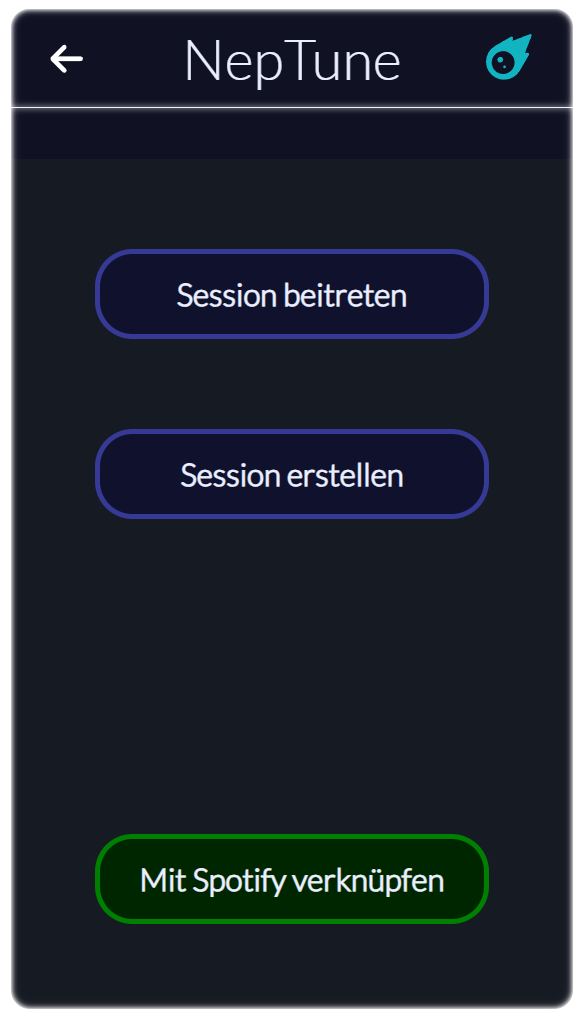
\includegraphics[width=5.5cm]{LATEX/Pflichtenheft/GraphicDesigns/startPage.png}
      \caption{startPage}
   \end{minipage}
   \hspace{2cm}% Abstand zwischen Bilder
   \begin{minipage}[b]{.4\linewidth} % [b] => Ausrichtung an \caption
      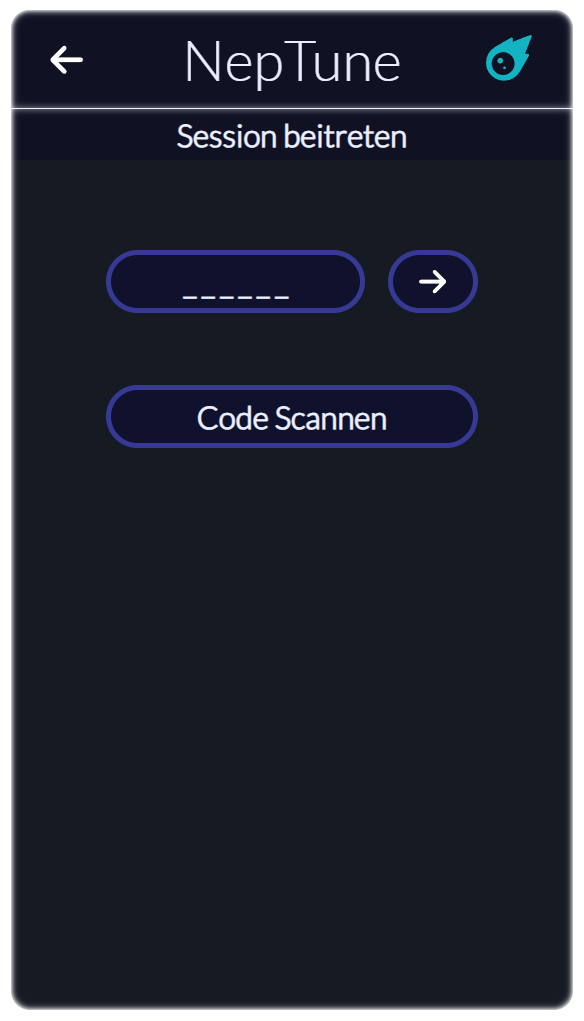
\includegraphics[width=5.5cm]{LATEX/Pflichtenheft/GraphicDesigns/userJoinGroupPage.png}
      \caption{userJoinGroupPage}
   \end{minipage}
   
   \begin{minipage}[b]{.4\linewidth} % [b] => Ausrichtung an \caption
      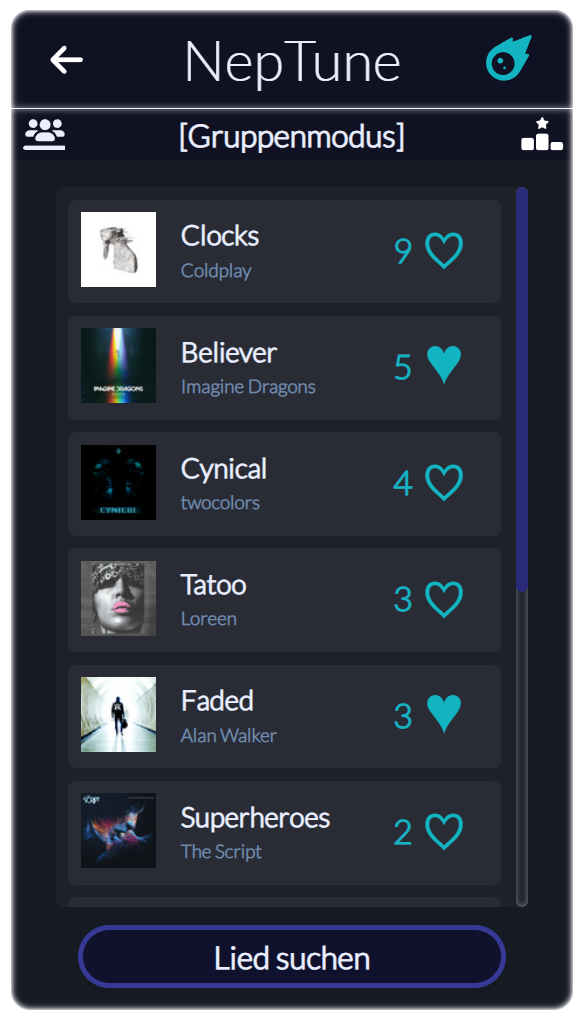
\includegraphics[width=5.5cm]{LATEX/Pflichtenheft/GraphicDesigns/userVotePage.png}
      \caption{userVotePage}
   \end{minipage}
   \hspace{2cm}% Abstand zwischen Bilder
   \begin{minipage}[b]{.4\linewidth} % [b] => Ausrichtung an \caption
      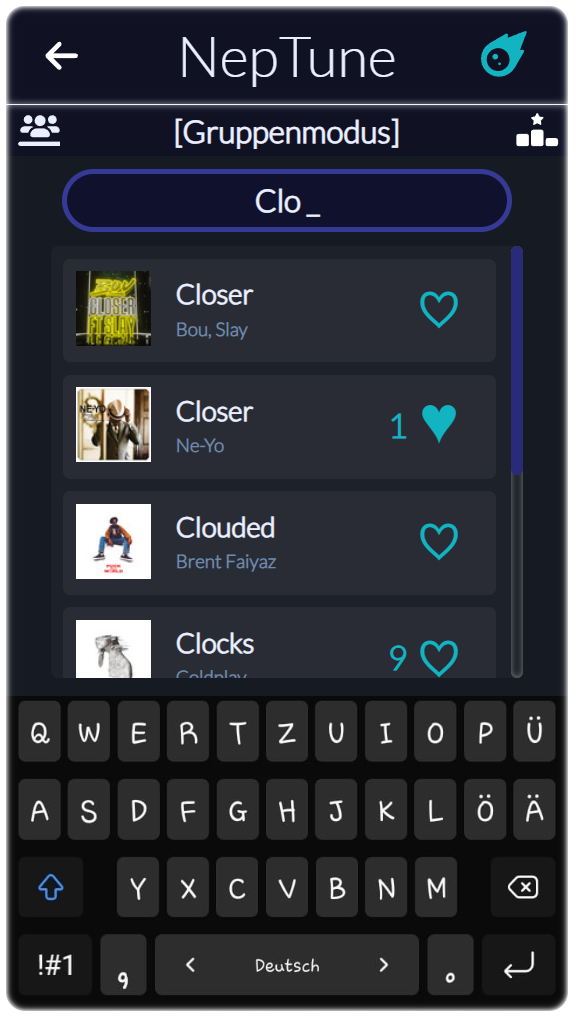
\includegraphics[width=5.5cm]{LATEX/Pflichtenheft/GraphicDesigns/userSearchPage.png}
      \caption{userSearchPage}
   \end{minipage}
\end{figure}

\begin{figure}
   \begin{minipage}[b]{.4\linewidth} % [b] => Ausrichtung an \caption
      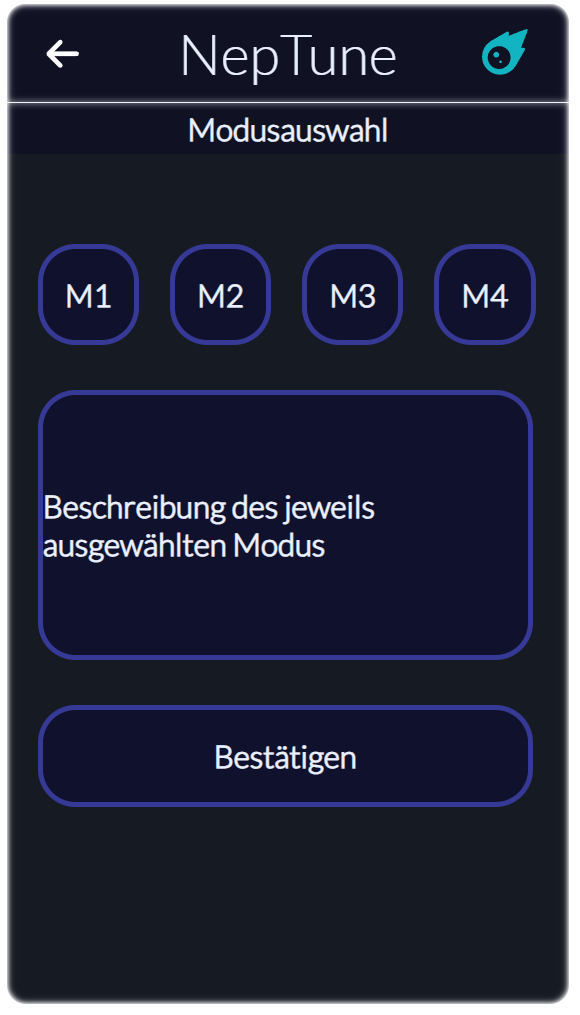
\includegraphics[width=6cm]{LATEX/Pflichtenheft/GraphicDesigns/hostModusSelectPage.png}
      \caption{hostModusSelectPage}
   \end{minipage}
   \hspace{2cm}% Abstand zwischen Bilder
   \begin{minipage}[b]{.4\linewidth} % [b] => Ausrichtung an \caption
      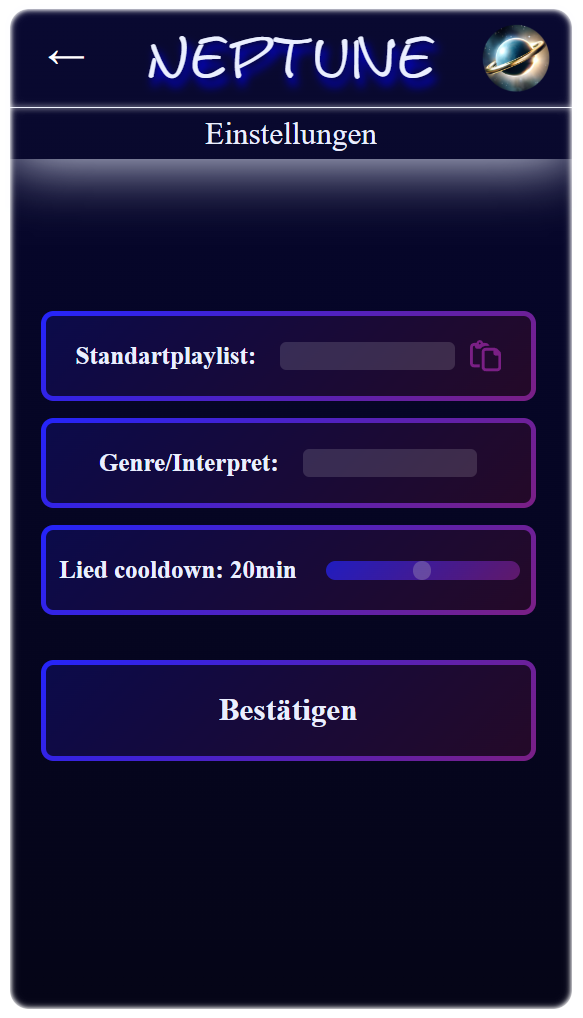
\includegraphics[width=6cm]{LATEX/Pflichtenheft/GraphicDesigns/hostModusSettingsPage.png}
      \caption{hostModusSettingsPage}
   \end{minipage}
   
   \begin{minipage}[b]{.4\linewidth} % [b] => Ausrichtung an \caption
      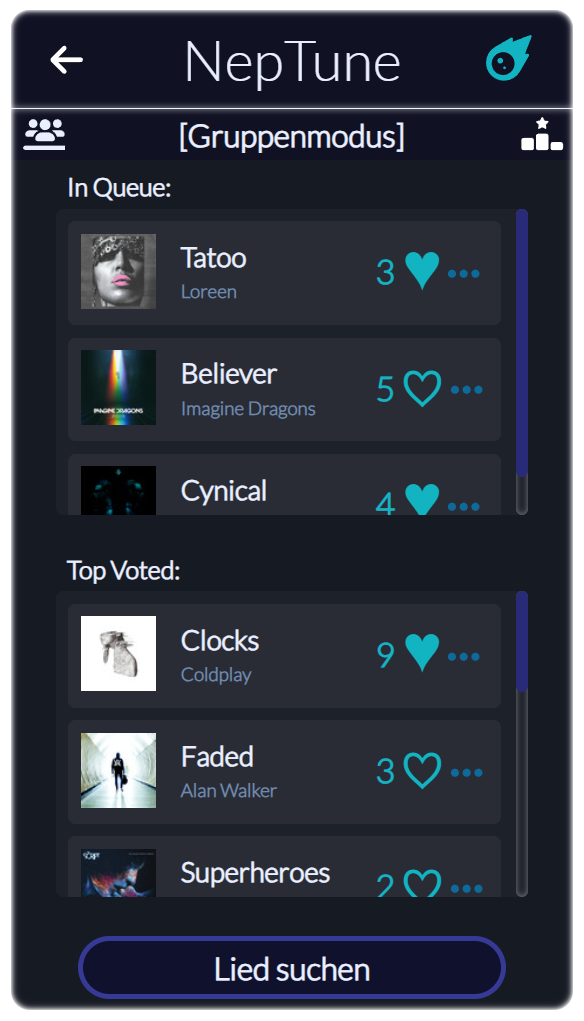
\includegraphics[width=6cm]{LATEX/Pflichtenheft/GraphicDesigns/hostControlPage.png}
      \caption{hostControlPage}
   \end{minipage}
   \hspace{2cm}% Abstand zwischen Bilder
   \begin{minipage}[b]{.4\linewidth} % [b] => Ausrichtung an \caption
      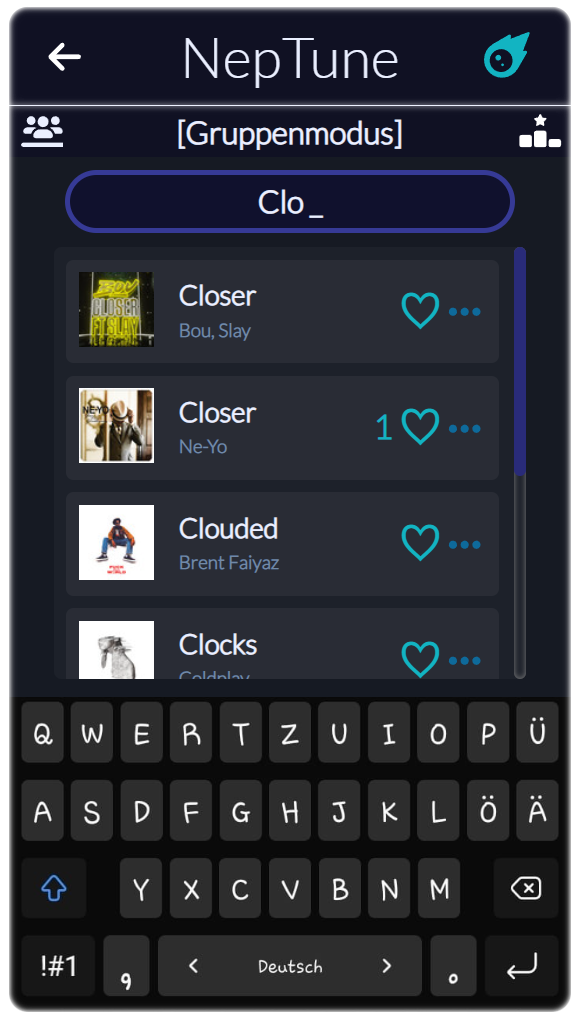
\includegraphics[width=6cm]{LATEX/Pflichtenheft/GraphicDesigns/hostSearchPage.png}
      \caption{hostSearchPage}
   \end{minipage}
\end{figure}

\begin{figure}
   \begin{minipage}[b]{.4\linewidth} % [b] => Ausrichtung an \caption
      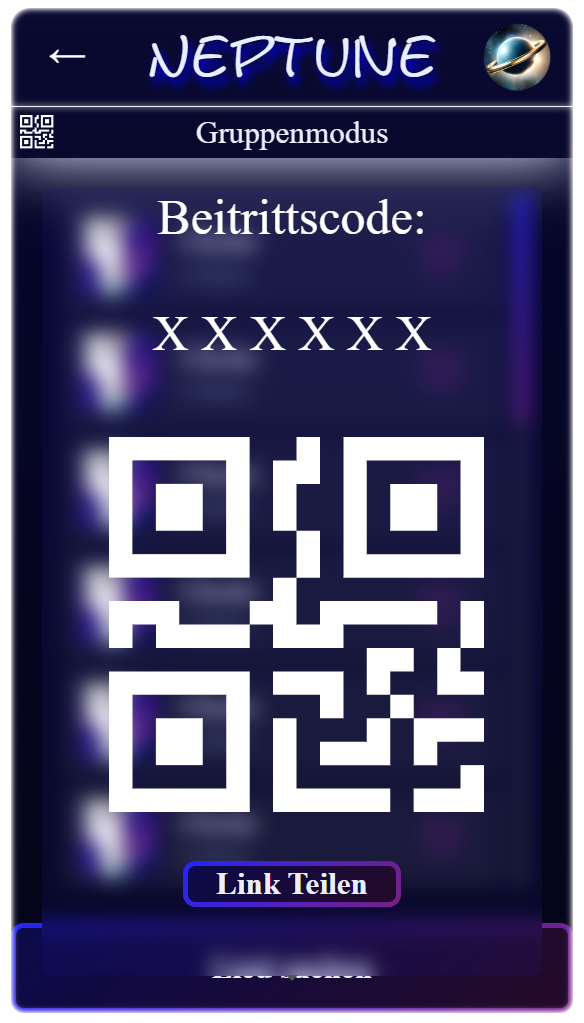
\includegraphics[width=6cm]{LATEX/Pflichtenheft/GraphicDesigns/shareLinkPopUpPage.png}
      \caption{shareLinkPopUpPage}
   \end{minipage}
\end{figure}

Spare Text:

Um ein übersichtliches Startmenü zu gewährleisten kann der Nutzer nur zwischen den Optionen "Gruppe beitreten" und "Gruppe erstellen" wählen. 

Im Startmenü kann der Nutzer entweder über die Buttons in der Mitte einer Gruppe beitreten, oder eine Gruppe erstellen. Über den Zurück-Knopf oben links verlässt der Nutzer die App.

Auf der Nutzer Abstimmungsseite sieht der Nutzer lieder bereits von Gruppenmitglieder vorgeschlagen und geliked wurden. Zudem kann er Lieder liken, welche er noch nicht geliked hat. Durch klicken des Lieder suchen Buttons gelangt der Nutzer zur Liedersuche. Über den Zurück-Knopf oben links gelangt der Nutzer zurück zum Startmenü. Dieser Vorgang muss über ein Pop-Up Fenster bestätigt werden, da gleichseitig die Gruppe verlassen wird.




\chapter{Qualitätszielbestimmungen}
\label{chap:Qualitätszielbestimmungen}

\textbf{Korrekte Funktionalität}: Die korrekte Funktionalität der App muss gewährleistet sein. Maßgeblich zur Definition dieser korrekten Funktionalität ist dieses Pflichtenheft und insbesondere die Musskriterien aus dem Kapitel der Zielbestimmungen (\ref{sec:Zielbestimmungen:Musskriterien}).

\textbf{Benutzerfreundlichkeit}: Die App soll eine einfache und intuitive Benutzererfahrung bieten. Die Navigation innerhalb der App soll für alle Benutzer leicht verständlich sein, ohne dass diese eine Einführung in die App-Bedienung benötigen.

\textbf{Schnelligkeit}: Die App soll durch Reaktionsschnelligkeit ein flüssiges und ansprechendes Nutzungserlebnis ermöglichen. Jede Schaltflächenbedienung soll eine unmittelbares Feedback für den Benutzer auslösen, ohne dass dieser eine Wartezeit bemerkt, solange das Endgerät hinreichend aktuell ist.

\textbf{Sicherheit der Benutzerdaten}: Es ist essentiell, dass die persönlichen Daten der Benutzer geschützt sind. Jegliche Interaktion mit und Datenverarbeitung durch die App muss datenschutzkonform sein und Datensicherheit bieten.

\textbf{Stabilität und Zuverlässigkeit}: Die App muss robust sein und selbst unter Last und bei mäßig vielen gleichzeitigen Benutzern stabil bleiben, sodass Abstürze oder unerwartete Fehler weitestgehend vermieden werden.

\textbf{Wartbarkeit und Portierungsmöglichkeiten}: Die Architektur der App soll gut wartbar sein, um zukünftige Anpassungen oder Erweiterungen zu ermöglichen. Zudem soll die Architektur die Möglichkeit zur verhältnismäßig einfachen Portierung der App auf andere mobile Betriebssysteme wie iOS bieten. 

\textbf{Grundsätzliches zur Qualität}: Diese Qualitätszielbestimmungen werden während allen Projektphasen beachtet und in der Qualitätssicherungsphase intern abgenommen. Die Qualität der App besitzt während allen Projektphasen einen sehr hohen Stellenwert: Sie wird stets als Priorität betrachtet und in der Qualitätssicherungsphase abschließend und eingehend geprüft.



\chapter{Testfälle und -szenarien}
\label{chap:Tests}

In diesem Kapitel werden alle Testfälle und -szenarien definiert, die einen oder mehrere Benutzer des fertiggestellten Produkts durchgeführt werden. Die hier definierten Testfälle sollen deshalb explizit keine technischen Funktionalitäten testen, die ausreichend detailliert erst während der Entwurfsphase festgelegt werden. Solche technischen Funktionalitäten werden durch Unittests abgedeckt, die während der Entwurfs- und Implementierungsphase entworfen und implementiert werden.

\section{Testfälle}
\label{sec:Tests:Testfälle}

Testfälle sind Tests zu aus Benutzersicht atomaren Vorgängen. Jeder Testfall bezieht sich also auf eine einzelne atomare Benutzereingabe. Eine solche Benutzereingabe besteht entweder aus einem einzelnen Touch-Eingabe oder einer inhaltlich sehr stark zusammenhängenden Folge von Touch-Eingaben, die als atomar betrachtet wird. (Jede Grundfunktionalität der App wird durch mindestens einen Testfall überprüft.)

\begin{itemize}
    \item Starten und Laden der App
    \item Verlassen der App
    \item Beenden der App
    \item Gruppenbeitritt beginnen
    \item Gruppenbeitritt verlassen
    \item Eingabe des Zugangscodes zum Gruppenbeitritt
    \item Veranlassen des tatsächlichen Gruppenbeitritts
    \item Verlassen der Gruppe
    \item Abstimmen für einen Song
    \item Öffnen der Songsuche
    \item Verlassen der Songsuche
    \item Suchen eines Songs
    \item Hinzufügen eines Songs
    \item Gruppenerstellung beginnen
    \item Gruppenerstellung verlassen (Modus-Eigenschaften)
    \item Auswählen des Modus (evt. noch nicht atomar genug)
    \item Bestätigung des Modus
    \item Gruppenerstellung verlassen (Modus-Details)
    \item Auswählen der Details des Modus
    \item Bestätigung der Details des Modus
    \item Gruppe löschen
    \item Lied abspielen
    \item .......?
\end{itemize}

\section{Testszenarien}
\label{sec:Tests:Testszenarien}

Testszenarien sind eine Folge von atomaren Testfällen, die beispielhaft eine Benutzerinteraktion durchspielen.

\subsection{Testszenario 1: Eine simple Benutzung}
\label{subsec:Tests:Testszenarien:1}
Zwei Nutzer, ein Host und ein normaler Benutzer (???), erstellen eine Gruppe, bzw. treten einer Gruppe bei, schlagen einen Song vor und spielen diesen ab.

\begin{itemize}
    \item Starten und Laden der App
    \item ......
\end{itemize}



\chapter{Entwicklungsumgebung}
\label{chap:Entwicklungsumgebung}

\section{Software}
\label{sec:Entwicklungsumgebung:Software}

\begin{itemize}
    \item Entwicklung
    \begin{itemize}
        \item Android Studio Giraffe (2022.3.1)
    \end{itemize}
    
    \item Versionsverwaltung
    \begin{itemize}
        \item GitHub
    \end{itemize}

    \item Modellierung
    \begin{itemize}
        \item Creately
    \end{itemize}

    \item Sonstige Software
    \begin{itemize}
        \item LATEX (Dokumentation)
        \item ...
    \end{itemize}
    
\end{itemize}

\section{Hardware}
\label{sec:Entwicklungsumgebung:Hardware}

\begin{itemize}
    \item Diverse Standard PCs
    \item Diverse Android Smartphones mit mindestens Android 7.0
\end{itemize}


\chapter{Begriffserklärungen}
\label{chap:Begriffserklärungen}


\section{}
\end{document}
